\begin{appendix}
\label{appe}
\chapter{Appendix}
\section {Customizing the Aurora Core}
\label{coregen}
Aurora core can be customized according the application. An example settings screen shot is shown below.  Refer figure \ref{auroraIP1} to figure \ref{auroraIP3} for details.
\begin{figure}[H]
  \centering
   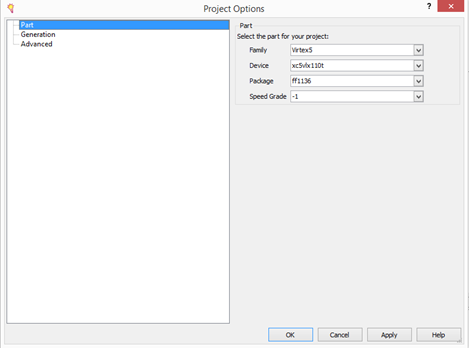
\includegraphics[scale=1]{./figs/auroraIP1}
  \caption{\textbf{Part selection for core generation}}
  \label{auroraIP1}
\end{figure}

\begin{figure}[H]
  \centering
   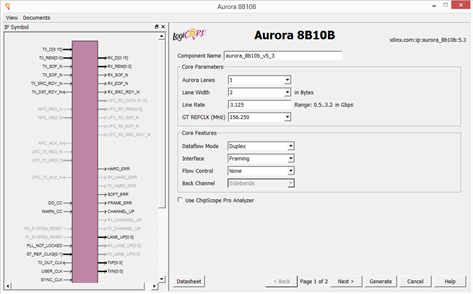
\includegraphics[scale=1]{./figs/auroraIP2}
  \caption{\textbf{Customizing Aurora core page 1}}
  \label{auroraIP2}
\end{figure}

\begin{figure}[H]
  \centering
   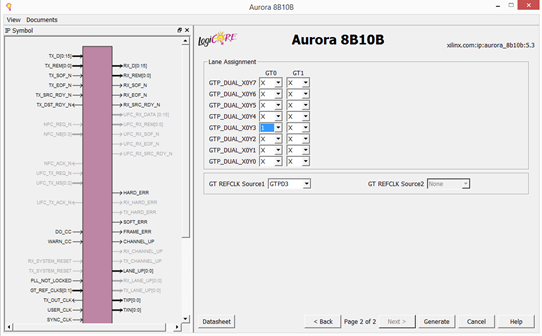
\includegraphics[scale=0.8]{./figs/auroraIP3}
  \caption{\textbf{Customizing Aurora core page 2}}
  \label{auroraIP3}
\end{figure}

\begin{enumerate}
	\item{Open Xilinx core generator.}
	\item{Create new project.}
	\item{Make the setting as shown}
	\item{Double click Communication and Networking $>$ Serial Interface $>$ Aurora 8B10B}
	\item{Make settings according to above figure}
	\item{Click generate.}
	\item{Open the generated core in Xilinx ISE. This generated design has an example test bench. This example design has a frame generator and a frame check module.}
\end{enumerate}

\section {CONNECT NoC generator}
\label{CONNECT}
CONNECT is a flexible RTL generator for fast, FPGA-friendly Networks-on-Chip. This website serves as a front-end to CONNECT's network generation engine, which is primarily based on Bluespec System Verilog. All networks generated through CONNECT consist of fully synthesizable Verilog.  CONNECT supports a variety of common network topologies, as well as custom user-specified networks. A variety of network and router parameters, such as router type, pipe-lining options, the number of virtual channels or allocator type,  allow the user to further customize the network and trade-off between resource  usage and performance.  For license information please see the LICENSE file.

All necessary files to implement a working network are located in this directory.  For networks with credit-based flow control the top module is called "mkNetwork" and is located in the mkNetwork.v \\ file. For networks with peek flow control the top module is called mkNetworkSimple and is located in the mkNetworkSimple.v \\ file. Both the mkNetwork and mkNetworkSimple module interfaces consist of a set of ports used for sending and receiving flits and flow control information.  The credit-based and peek-based networks share the same interface for sending and receiving flits, but offer different flow-control interfaces, which are detailed below. 

\begin{enumerate}
\item{EN\_send\_ports\_$<$P$>$\_putFlit input wire: Assert when sending a flit to indicate send\_ports\_P\_putFlit\_flit\_in carries valid data.}
\item{send\_ports\_$<$P$>$\_putFlit\_flit\_in input bus}
\item{EN\_send\_ports\_$<$P$>$\_getNonFullVCs input wire: indicates sender is ready to receive a credit.}
\item{send\_ports\_$<$P$>$\_getNonFullVCs, output bus, that carries a bit-mask indicating which VCs have available buffers space (i.e. are non-Full). MSB corresponds to the highest VC and LSB corresponds to the lowest VC. For non-VC networks this signal is a single bit.}
\item{EN\_recv\_ports\_P\_getFlit input wire: Assert when ready to receive an incoming flit}
\item{Recv\_ports\_P\_getFlit output bus}
\end{enumerate}

CONNECT-generated networks that use Peek flow control offer a simpler interface. Instead of maintain and exchanging credits, network clients simply need to check if the buffer they intend to inject into is not full by checking the send\_ports\_$<$P$>$\_getNonFullVCs signal. In the case of VC-based networks they need to check the specific bit that corresponds to the VC that the flit belongs to.\\

\section {Partitioned Network with Aurora 8B10B IP: Project Directory Structure}
\label{CONNECTAurora}
custom\_TB.v \\
	| ---- Example\_design\_1\_i.v \\
	|       		|-------clock)module\_i.v \\
	|		|-------standard\_cc\_module.v \\
	|		|-------reset\_logic.v \\
	|		|-------aurora\_module\_i\_3
	|		|		|-----aurora\_lane\_0\_i.v \\
	|		|		|		|-----lane\_init\_sm\_i.v \\
	|		|		|		|-----chbond\_count\_dec\_i.v \\
	|		|		|		|-----sym\_gen\_i.v \\
	|		|		|		|-----sym\_dec\_i.v \\
	|		|		|		|-----err\_detect\_i.v \\
	|		|		|-----gtp\_wrapper.v \\
	|		|		|		|-----GTP\_TILE\_INST.v \\
	|		|		|-----global \_logic.v \\
	|		|		|		|-----channel\_init\_sm\_i.v \\
	|		|		|		|-----idle\_and\_ver\_gen\_i.v \\
	|		|		|		|-----channel\_err\_detect\_i.v \\
	|		|		|-----tx\_ll\_i.v \\
	|		|		|		|-----tx\_ll\_datapath\_i
	|		|		|		|-----tx\_ll\_controlpath\_i
	|		|		|-----rx\_ll\_i.v \\
	|		|		|		|-----rx\_ll\_pdu\_datapath\_i
	|		|-------aurora\_module\_i\_4
	|		|		|-----aurora\_lane\_0\_i.v \\
	|		|		|		|-----lane\_init\_sm\_i.v \\
	|		|		|		|-----chbond\_count\_dec\_i.v \\
	|		|		|		|-----sym\_gen\_i.v \\
	|		|		|		|-----sym\_dec\_i.v \\
	|		|		|		|-----err\_detect\_i.v \\
	|		|		|-----gtp\_wrapper.v \\
	|		|		|		|-----GTP\_TILE\_INST.v \\
	|		|		|-----global \_logic.v \\
	|		|		|		|-----channel\_init\_sm\_i.v \\
	|		|		|		|-----idle\_and\_ver\_gen\_i.v \\
	|		|		|		|-----channel\_err\_detect\_i.v \\
	|		|		|-----tx\_ll\_i.v \\
	|		|		|		|-----tx\_ll\_datapath\_i.v \\
	|		|		|		|-----tx\_ll\_controlpath\_i.v \\
	|		|		|-----rx\_ll\_i.v \\
	|		|		|		|-----rx\_ll\_pdu\_datapath\_i.v \\
	|		|------dut1-mkSimpleNetwork\_1.v \\

	|		|------- Example\_design\_2\_i.v \\
	|       	|------- clock\_module\_i.v \\
	|		|------- standard\_cc\_module.v \\
	|		|------- reset\_logic.v \\
	|		|------- aurora\_module\_i\_2
	|		|		|-----aurora\_lane\_0\_i.v \\
	|		|		|		|-----lane\_init\_sm\_i.v \\
	|		|		|		|-----chbond\_count\_dec\_i.v \\
	|		|		|		|-----sym\_gen\_i.v \\
	|		|		|		|-----sym\_dec\_i.v \\
	|		|		|		|-----err\_detect\_i.v \\
	|		|		|-----gtp\_wrapper.v \\
	|		|		|		|-----GTP\_TILE\_INST.v \\
	|		|		|-----global \_logic.v \\
	|		|		|		|-----channel\_init\_sm\_i.v \\
	|		|		|		|-----idle\_and\_ver\_gen\_i.v \\
	|		|		|		|-----channel\_err\_detect\_i.v \\
	|		|		|-----tx\_ll\_i.v \\
	|		|		|		|-----tx\_ll\_datapath\_i
	|		|		|		|-----tx\_ll\_controlpath\_i
	|		|		|-----rx\_ll\_i.v \\
	|		|		|		|-----rx\_ll\_pdu\_datapath\_i
	|		|-------aurora\_module\_i\_1
	|		|		|-----aurora\_lane\_0\_i.v \\
	|		|		|		|-----lane\_init\_sm\_i.v \\
	|		|		|		|-----chbond\_count\_dec\_i.v \\
	|		|		|		|-----sym\_gen\_i.v \\
	|		|		|		|-----sym\_dec\_i.v \\
	|		|		|		|-----err\_detect\_i.v \\
	|		|		|-----gtp\_wrapper.v \\
	|		|		|		|-----GTP\_TILE\_INST.v \\
	|		|		|-----global \_logic.v \\
	|		|		|		|-----channel\_init\_sm\_i.v \\
	|		|		|		|-----idle\_and\_ver\_gen\_i.v \\
	|		|		|		|-----channel\_err\_detect\_i.v \\
	|		|		|-----tx\_ll\_i.v \\
	|		|		|		|-----tx\_ll\_datapath\_i.v \\
	|		|		|		|-----tx\_ll\_controlpath\_i.v \\
	|		|		|-----rx\_ll\_i.v \\
	|		|		|		|-----rx\_ll\_pdu\_datapath\_i.v \\
	
\newpage	
\section {Python code for NoC Partitioning}
\label{pythonCode}
Note: The following code segment is just to give an idea of the partitioning approach. A few minor modification are needed to execute and generate the partition NoC. I wish to sincerely thank Yatish Turakhia for providing me with the original python script for NoC partitioning and allowing me to use and modify for my project thesis work.  
\lstinputlisting[language=Python]{mkNetworkScript4x4_0.py}

\newpage	
\section {Quasi-SERDES Link Module Verilog HDL}
\label{serdes}
Note: This Verilog code segment should give an idea behind its implementation.
\lstinputlisting[language=Verilog]{phy.v}


\newpage	
\section {Top Level NoC after partitioning}
\label{NoCTop}
Note: This is the top level Verilog module to demonstrate the instantiation on partitioned NoC. The module can be used for simulating the design and comparing the results with un-partitioned NoC. The original CONNECT test bench can be used to test this partitioned top level design. 
\lstinputlisting[language=Verilog]{mkNetworkSimple_top.v}


\end{appendix}